\documentclass[a4paper,oneside,phd,etd]{BYUPhys}
% The BYUPhys class is for producing theses and dissertations
% in the BYU Department of Physics and Astronomy.  You can supply
% the following optional arguments in the square brackets to
% specify the thesis type:
%
%   senior  : Produces the senior thesis preliminary pages (default)
%   honors  : Produces the honors thesis preliminary pages
%   masters : Produces the masters thesis preliminary pages
%   phd     : Produces the PhD dissertation preliminary pages
%
% The default format is appropriate for printing, with blank pages
% inserted after the preliminary pages in twoside mode so you can
% send it directly to a two-sided printer. However, for ETD
% submission the blank pages need to be removed from the final output.
% The following option does this for you:
%
%   etd     : Produces a copy with no blank pages in the preliminary section.
%             Remove this option to produce a version with blank pages inserted
%             for easy double sided printing.
%
% The rest of the class options are the same as the regular book class.
% A few to remember:
%
%   oneside : Produces single sided print layout (recommended for theses less than 50 pages)
%   twoside : Produces double sided print layout (the default if you remove oneside)
%
% The BYUPhys class provides the following macros:
%
%   \makepreliminarypages : Makes the preliminary pages
%   \clearemptydoublepage : same as \cleardoublepage but doesn't put page numbers
%                           on blank intervening pages
%   \singlespace          : switch to single spaced lines
%   \doublespace          : switch to double spaced lines
%
% --------------------------- Load Packages ---------------------------------

% The graphicx package allows the inclusion of figures.  Plain LaTeX and
% pdfLaTeX handle graphics differently. The following code checks which one
% you are compiling with, and switches the graphicx package options accordingly.
\usepackage{ifpdf}
\ifpdf
  \usepackage[pdftex]{graphicx}
\else
  \usepackage[dvips]{graphicx}
\fi

%%%%%%%%%%%%%%%%%%%%%%%%%%%%%%%%%%%%%%%%%%%%%%%%%%%%%%%%%%%%%%%%%%
% Edited : Beeshanga
%
% If you need to include any code in the text use this package
% \usepackage{listings}
% It can be used to make key words bold, add colours, etc. Refer
% to http://en.wikibooks.org/wiki/LaTeX/Packages/Listings for
% more information.
%
% For theorems, propositions, proofs and assumptions use this
% package
% \usepackage{amsthm}
% For more information refer to the following website
% http://en.wikibooks.org/wiki/LaTeX/Theorems
%
%%%%%%%%%%%%%%%%%%%%%%%%%%%%%%%%%%%%%%%%%%%%%%%%%%%%%%%%%%%%%%%%%%

% The fancyhdr package allows you to easily customize the page header.
% The settings below produce a nice, well separated header.
\usepackage{fancyhdr}
  \fancyhead{}
  \fancyhead[LO]{\slshape \rightmark}
  \fancyhead[RO,LE]{\textbf{\thepage}}
  \fancyhead[RE]{\slshape \leftmark}
  \fancyfoot{}
  \pagestyle{fancy}
  \renewcommand{\chaptermark}[1]{\markboth{\chaptername \ \thechapter. #1}{}}
  \renewcommand{\sectionmark}[1]{\markright{\thesection \ #1}}


% The cite package cleans up the way citations are handled.  For example, it
% changes the citation [1,2,3,6,7,8,9,10,11] into [1-3,6-11].  If your advisor
% wants superscript citations, use the overcite package instead of the cite package.
\usepackage{cite}

% The makeidx package makes your index for you.  To make an index entry,
% go to the place in the book that should be referenced and type
%  \index{key}
% An index entry labeled "key" (or whatever you type) will then
% be included and point to the correct page.
%\usepackage{makeidx}
%\makeindex

% The url package allows for the nice typesetting of URLs.  Since URLs are often
% long with no spaces, they mess up line wrapping.  The command \url{http://www.physics.byu.edu}
% allows LaTeX to break the url across lines at appropriate places: e.g. http://www.
% physics.byu.edu.  This is helpful if you reference web pages.

\usepackage[hyphens]{url}
\urlstyle{same}
\usepackage{cite}

%\usepackage{url}
%\urlstyle{rm}

% If you have a lot of equations, you might be interested in the amstex package.
% It defines a number of environments and macros that are helpful for mathematics.
% We don't do much math in this example, so we haven't used amstex here.
\usepackage{amsmath}
\usepackage{amssymb}
\usepackage{subfigure}
\usepackage{cite}
\usepackage{amsxtra}
\usepackage{amsfonts}
\usepackage{graphicx}
\usepackage{multirow} % This is package for multi-rows in tables added on 7th July 2009 by Arif
%\usepackage{setspace}

% The caption package allows us to change the formatting of figure captions.
% The commands here change to the suggested caption format: single spaced and a bold tag
\usepackage[labelfont=bf,labelsep=colon]{caption}%[2008/04/01]
 \DeclareCaptionFormat{suggested}{\singlespace#1#2#3\par\doublespace}
 \captionsetup{format=suggested}


\usepackage{array}
\usepackage{multirow}
\usepackage{verbatim}
\usepackage{enumerate}

% Defining the symbols




% The hyperref package provides automatic linking and bookmarking for the table
% of contents, index, equation references, and figure references.  It must be
% included for the BYU Physics class to make a properly functioning electronic
% thesis.  It should be the last package loaded if possible.
%
% To include a link in your pdf use \href{URL}{Text to be displayed}.  If your
% display text is the URL, you probably should use the \url{} command discussed
% above.
%
% To add a bookmark in the pdf you can use \pdfbookmark.  You can look up its usage
% in the hyperref package documentation
\usepackage[bookmarksnumbered,pdfpagelabels=true,plainpages=false,colorlinks=true,
            linkcolor=black,citecolor=red,urlcolor=blue]{hyperref}
\hypersetup{breaklinks=true}

% My custom packages
\usepackage{float}


% ------------------------- Fill in these fields for the preliminary pages ----------------------------
%
% For Senior and honors this is the year and month that you submit the thesis
% For Masters and PhD, this is your graduation date
  \Year{2019}
  \Month{June 7th,}
  \Author{James Ridey}

% If you have a long title, split it between two lines. The \TitleBottom field defines the second line
% A two line title should be an "inverted pyramid" with the top line longer than the bottom.
  \TitleTop{Reduction of neural network complexity through}
  \TitleBottom{stochastic numbers} % edited Beeshanga
 \DegreeTitle{Bachelor of Engineering
 \\ Software Engineering} % edited Beeshanga

% Your research advisor
 \Advisor{Supervisor: Associate Professor Tara Hamilton}

% The department undergraduate research coordinator
%  \UgradCoord{A}

% The representative of the department who will approve your thesis (usually the chair)
%  \DepRep{B}

% Acknowledge those who helped and supported you

  \Acknowledgments{
  \vspace{-1.5cm}
    \noindent I would like to acknowledge and thank, Tara Hamilton and Alan Kan for their support and advice during my thesis.
  }


% The title of the department representative
%  \DepRepTitle{Chair}
  \Statement{
    \noindent I, James Ridey, declare that this report, submitted as part of the requirement for the award of Bachelor of Engineering in the School of Engineering, Macquarie University, is entirely my own work unless otherwise referenced or acknowledged. This document has not been submitted for qualification or assessment at any academic institution.
    \vspace{0.5cm}

    \noindent     Student's Name: James Ridey

    \vspace{0.25cm}

    \noindent Student's Signature: James Ridey

    \vspace{0.25cm}

    \noindent     Date: 7/6/2019
    }

% The text of your abstract
\Abstract{
\vspace{-1.5 cm}
Neural networks considered a core foundation of machine learning, has recently ballooned into a large framework that requires vast amounts of computing resources and time. Here, we examine how to improve these networks, hoping to achieve networks that can calculate the same result with less training time and/or resources using, ideas such as stochastic numbers and probabilistic results.
}



% Statement of Candidate



\fussy

\begin{document}

 % Start page counting in roman numerals
 \frontmatter

 % This command makes the formal preliminary pages.
 % You can comment it out during the drafting process if you want to save paper.

 \makepreliminarypages


%\clearemptydoublepage
\doublespace
%\include{Publications/publications}

% \clearemptydoublepage
%\include{Organization/organization}

 \clearemptydoublepage
\singlespace
 % Make the table of contents.
 \tableofcontents

\clearemptydoublepage
% Make the list of figures
\listoffigures

\clearemptydoublepage
% Make the list of tables
%\listoftables

\clearemptydoublepage

% Start regular page counting at page 1
\mainmatter
%
\chapter{Introduction}
\label{chap:Introduction}


\section{Neural networks: introduction}
Neural networks are the core structure of what many believe to be the next step in computing, machine learning. We are starting to see machine learning used to solve problems that originally were only able to be solved by people. However, all this machine learning comes at a cost, machine learning needs vast amounts of data to learn and thus large amounts of computing resources, electricity, time and even the best machine learning models work within a narrow, controlled set of inputs, anything outside this "range" are misclassified, in other words, machine learnings models are sensitive to noise and not general enough.

My thesis details, my efforts to try and find a way to reduce machine learning complexity or finding a way to make machine learning models more tolerant to noise. The preliminary work done in this thesis relates to trying to use stochastic numbers with the Tensorflow machine learning framework on the MNIST dataset to try and find ways to reduce complexity.

\chapter{Background and Related Work}
\label{chap:LitReview}

\section{Neural networks: explanation}
Neural networks are a very rough simulation of how the neurons in a human brain actually work, they have been researched since the 1960s\cite{neural-network-history} but at the time we did not have the computing power necessary to run these large neural networks and thus progress was halted until around such time as 1970-1980's when backpropagation was discovered making neural network training much more efficient and parallel computing system was also starting to kick off.

The most common form of a neural network in the feedforward model where the inputs are passed to the neural network and it outputs an answer. The feedforward model consists of an input layer, hidden layers and an output layer each of these layers are composed of varying amounts of neurons depending on the complexity of the data that is trying to be learned. More models of neural networks exist which aim to memorise or improve the feedforward model, however, the feedforward model is incredibly ubiquitous and is the main driving force behind machine learning in the industry. 

To understand what each layer in a neural network is doing, it is first necessary to understand what a neuron is doing. A neuron is comprised of inputs, a set of weights, one output and an activation function, as shown below.
\begin{figure}[H]
\centering
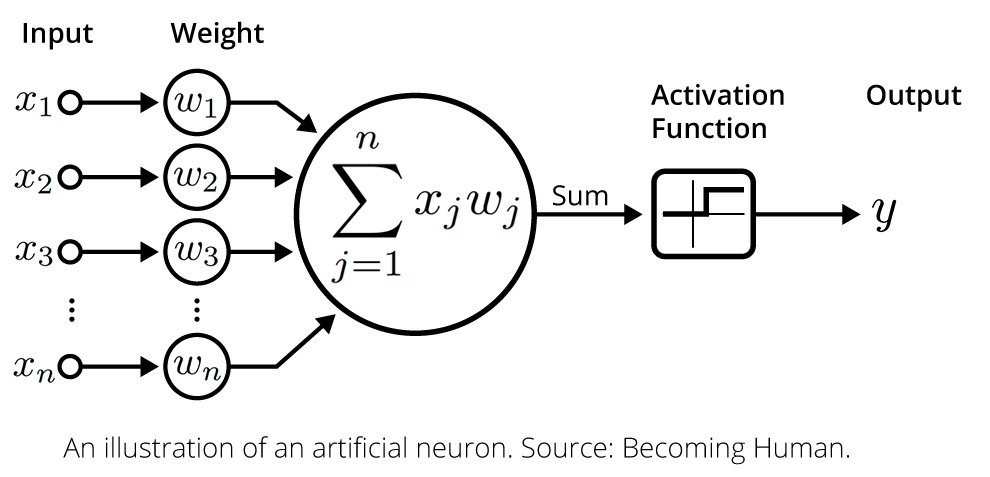
\includegraphics[width=8cm]{pictures/neuron_model.png}
\caption{Neuron model\cite{fig:neuron_model}.}
\label{fig:neuron_model}
\end{figure}

Neurons are fed a set of data through its inputs which are multiplied by a specific weight, all of these numbers are then added up and fed to an activation function. An activation function is a function that maps the input to a value between 0 and 1, a commonly used activation function is the sigmoid function, numbers in the positive infinity direction become increasingly closer to 1, while numbers in the negative infinity direction become increasing closer to 0.
\begin{figure}[H]
\centering
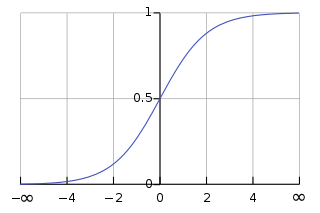
\includegraphics[width=8cm]{pictures/sigmoid.png}
\caption{Sigmoid graph\cite{fig:sigmoid}.}
\label{fig:sigmoid}
\end{figure}

Next is neural network layers varying based on the task you want to try an accomplish, some examples include convolutional layers which attempt to use neural networks on squares of pixels, dropout layers which randomly pick weights to drop to try and reduce overfitting and the most common layer used to most machine learning models, is the dense layer, in this layer every neuron connects to every other neuron in the previous layer.
\begin{figure}[H]
\centering
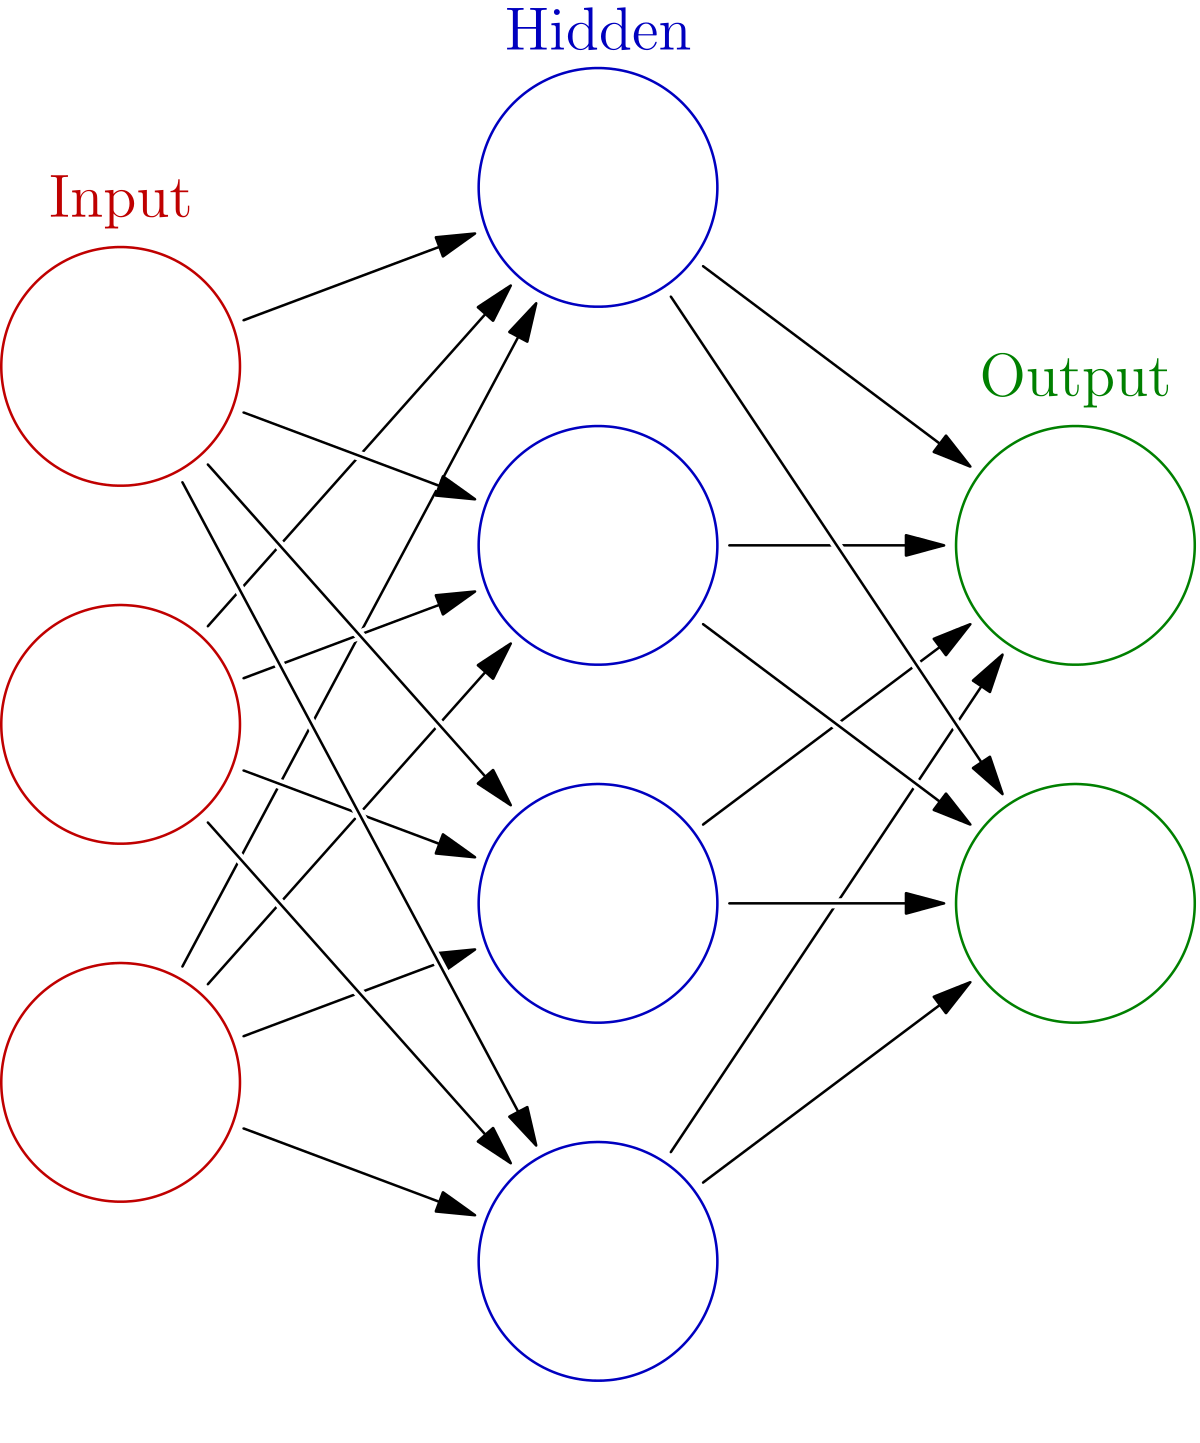
\includegraphics[width=8cm]{pictures/neural_network_model.png}
\caption{Neural network model\cite{fig:neural_network_model}.}
\label{fig:neural_network_model}
\end{figure}

Each circle in this figure represents a neuron and each line in this figure represents a connection between 2 neurons. By manipulating the weights in the neural network, we change what each neuron calculates and outputs as part of its activation function. In doing so, we now have a framework of which for any given input, the neural network can generate any output (given the right weights), regardless of the complexity of the output\cite{nielsen}. 

\subsection{Training}
The next question about neural networks is then how are the weights calculated for a given input. This is where training a neural network comes into play. The basic summary for how a neural network is trained is they are fed the input data, the error amount is calculated from the neural network output and then the weights are slowly adjusted to minimize the error rate. How this is all done is where the complexity of neural networks lie and why they take so long to train. One of the simplest algorithms that implements this is the stochastic gradient descent algorithm, which is a core component of many other machine learning algorithms like RMSprop, ADAM and AdaGrad (RMSprop being a commonly used algorithm and the one that was used in the majority of the MNIST tests). 

The gradient descent or GD works by measuring the gradient and trying to find a point at which the error is the lowest. The gradient being a measure of "how much the output of a function changes if you change the inputs a little bit"\cite{towards-data-science}.
The best way of explaining GD is with a hill climbing example, a blinded person is trying to find the highest point of a hill and so he starts by taking large steps to estimate where the steepest part of the hill is and then smaller and smaller steps until he finds the top of the hill. Applying this to machine learning, the error of the output of the machine learning model is compared with the actual values that are to be expected and this is the error amount, then the weights are changed are relatively "large" amount and the error is measured again and compared to the previous error, this is the gradient. This gradient is then used to estimate how big of a "step"/how much to adjust the weights by on the next iteration.
\begin{figure}[H]
\centering
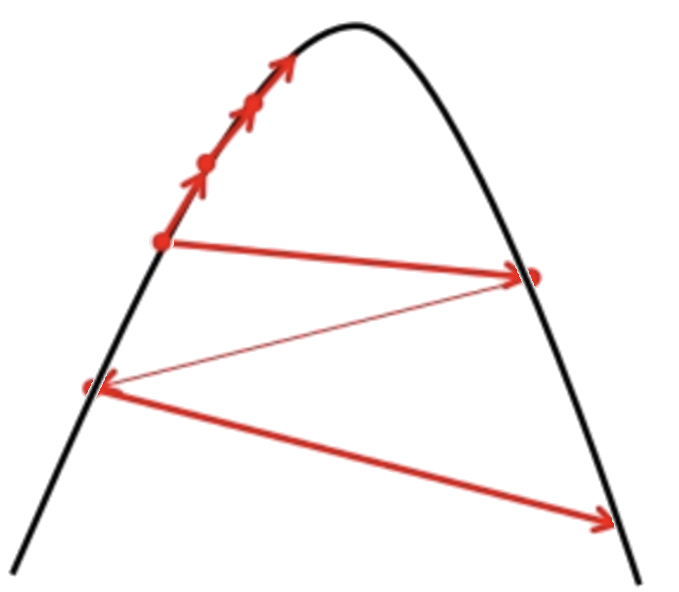
\includegraphics[width=6cm]{pictures/gradient.png}
\caption{Stochastic gradient example.
Y-Axis represents accuracy rate}
\label{fig:gradient}
\end{figure}

However in realities, there are much more dimensions to a machine learning model and secondly, there is not just one point that is the highest but multiple hills of varying heights, this is one of the many reasons why machine learning is hard. You can create simple machine learning algorithms that find a maximum point but not the global maximum point or the global maxima, you can also try and adjust how much you step by each amount but the best way, which requires all the computation power is a small stepping amount which tries all points on the "hills". 
\begin{figure}[H]
\centering
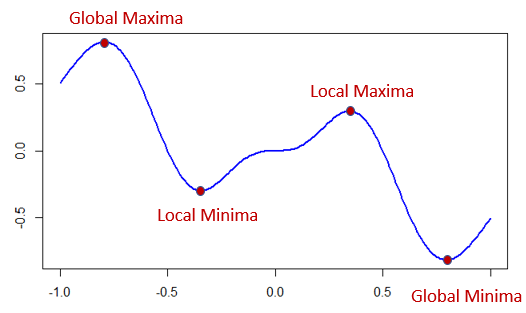
\includegraphics[width=10cm]{pictures/global_minima.png}
\caption{Global maxima example.
Y-Axis represents accuracy rate}
\label{fig:global_minima}
\end{figure}

\section{Stochastic computing}
Stochastic computing is a branch of computing that relies on probabilistic bit streams to calculate numbers, often relying on simple bit-wise operations. Every number in a stochastic computer is arranged as a probability of the ones and zeros in a continuous binary number stream. 

\subsection{Advantages of stochastic numbers}
There are 2 major advantages with this technique, one is that the system is extremely resistant to noise, flipping multiple bits in the stream will have very little effect or will only change the number minorly. The other major advantage is that certain operations have a simpler solution, for example in terms of multiplication on a conventional computer this would be an $n^2$ operation, however, on a stochastic computer, this is accomplished with an AND gate at a cost of $n$.

\subsection{Disadvantages of stochastic numbers}
However, the reason for stochastic computing not being proliferated is the inherent weakness which is the randomness of stochastic numbers. Stochastic numbers can never truly represent the number they are trying to calculate and thus need a large amount of sampling to "zone in" on the number being calculated.

Secondly is that while stochastic numbers have a simple analog for multiplication, the core of stochastic numbers like the PRNG (Pseudo-random number generator) for generating the random bit stream and decoding the bit stream by sampling do not have simple gate-level analogues and this is where stochastic numbers lose their advantage.

\section{Tensorflow}
Tensorflow\cite{tensorflow} is a machine learning framework primarily written in Python. It was released by Google under the Apache License 2.0 on November 9th, 2015. The Tensorflow network employs the idea of creating a neural network model which is then compiled before being handed off to the appropriate processing unit be it CPU, GPU or TPU, this is in contrast to other machine learning frameworks like PyTorch that generate their models dynamically on the fly which results in a small performance hit.

Tensorflow continues to grow in support with new frameworks like Kera that aim to simplify common operations and overall streamline the process and show no signs of stopping with a stable release only 2 months ago.

\section{PyTorch}
%TODO

\section{MNIST dataset}
The MNIST dataset\cite{lecun-website} is a commonly used dataset for machine learning that consists of 70,000 images of handwritten digits (60,000 training images and 10,000 test images) and the associated labels for each of these images. The dataset is commonly chosen due to its simplicity and many frameworks support it out of the box.
\begin{figure}[H]
\centering
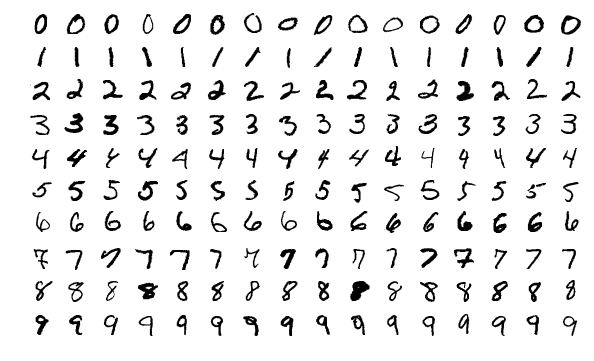
\includegraphics[width=8cm]{pictures/mnist.png}
\caption{Samples of the MNIST dataset\cite{fig:mnist}.}
\label{fig:mnist}
\end{figure}

Another common reason that MNIST is chosen is to demonstrate the accuracy of neural networks over more traditional statistical analysis such as linear classifiers and K-nearest neighbours, both of which score around an error rate of 12\% and 5\% respectively\cite{lecun-98} as compared to a simple neural network of 3 layers which can score around 3.05\%\cite{lecun-98}.

However this dataset is not without its faults, there are quite a number of images that are dubiously labelled.
\begin{figure}[H]
\centering
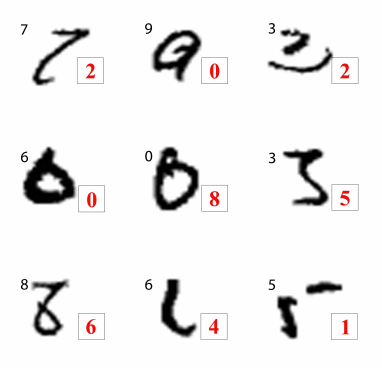
\includegraphics[width=8cm]{pictures/mnist_incorrect.png}
\caption{Samples of ambiguous digits\cite{fig:mnist_incorrect}.}
\label{fig:incorrect_mnist}
\end{figure}
The dataset is also often constructed as too small and too simple, consisting of only 70,000 images of greyscale images. Compared to datasets such as CIFAR10 which has the same amount of images but 32x32 colour images or another dataset like ImageNet consisting of 1,331,167 images, MNIST is certainly behind. However, MNIST has been used and is continued to be used as a way to quickly validate a machine learning algorithm before moving on to larger more complicated datasets that take much more time to compute.

\chapter{Results}
\section{Introduction}
The primary idea behind this thesis was to create a system where we could reliably compare 2 machine learning systems with one using stochastic computing and the other using convetional computing. While attempts have been made in building up entirely new systems from the ground up using stochastic computing to accomplish a machine learning task[cite]. There are little to none about system using stochastic computing inside of existing machine learning frameworks such that both systems are on an even playing field and you aren't comparing orange's and apple's. This was the goal we set out to accomplish, creating a system within an existing machine learning framework that could be applied to multiple datasets.

\section{The design}
Consdering that the goal of this thesis was to compare stochastic computing and conventional computing in the field of machine learning, the first step would be to implement the core part of a machine learning framework which is the matrix multiplication, this consists of three parts, the conversion from a binary floating point number to a stochastic number, the multiplication between the rows and columns of the matrix and finally the addition of each of the rows of the matrix. While most of thesis operations would be easy outside of a machine learning framework, implementing them within a machine learning framework requires a different way of thinking as each operation needs to be parrallizable and as such you are often restricted with what you are "allowed" to do, one such example of this is the heavy discouragement of the use of for loops[CITE] as used incorrectly this requires the data being processed to be passed between the GPU and CPU and will likely cause massive slowdowns.
\\\\
Each task had multiple ways of implementing the solution and each came with their own benefits and drawbacks, which will be detailed below.

\section{The conversion}
One of the secondary goals of this project was to create essentially a dropin machine learning layer that would use stochastic computing, this would mean that the dropin would have to convert the floating points it had received from the previous layer, convert it to a stochastic number for processing and then convert it back after the computation.
\\\\
The general operation for how a binary number is converted to a stochastic number is 
\begin{enumerate}
	\item Create a boolean array the size of the stochastic number you want
	\item For each boolean in the array, set it to the condition (value $\geq$ random\_float(0,1))
\end{enumerate}
This is further shown in the pseudocode below
\\\\
<code></code>\\
However in terms of a machine learning framework the following is done instead, 
\begin{enumerate}
	\item Take the matrix of floating points, and add an extra dimension to it
	\item Scale the size of the newly created dimensional such that it repeats each value for the size of the stochastic number
	\item Apply (value $\geq$ random\_float(0,1)) over the entire matrix
\end{enumerate}

This covers the general approach to converting binary numbers to stochastic numbers, converting them back means simply taking the mean of the entire array/matrix. However while this covers the general approach there are some nuances that need to be discussed. The first is the use of the random number generator, stochastic numbers are very sensitive to correlation[CITE] and so each random number must be generated separately fomr the other, while a general psuedorandom number generator (PRNG) will certainly do the trick, there has been studies showing better results can be achieved with a customised PRNG[CITE], we decided against going down this route as it would be complicated to integrate and ultimately detract form the goal of this thesis.
\\\\
Another nuace of this algorithm is the size of the stochastic number, having more bits in your stochastic number will ultimately improve its performance but it comes at the cost of memory (which can balloon very quickly with large matrixes) and
computational time. Plus after further investigation, we found that increasing the number of bits has diminising effects.
\\\\
<graph></graph>\\
As shown in the graph above, as the bits increase, the varience decreases but it reaches a point where the number of bits accounts for such a small change in the varience that it is ultimately not worth the memory or time. We did some research to try and find a way to have progressive accuracy woth stochastic computing but we unable to find and instances of such a case. And finally the last nuace is the range of the stochastic numbers as the conditional (value $\geq$ random\_float(0,1)) will give a range on the stochastic numbers between 0 and 1, there exists an alternative form for negative numbers where the conditional becomes (value+1/2 $\geq$ random\_float(0,1) essentially the -1 to 1 range of value is mapped between 0 and 1. However there are a few caveats with this, one is that now each bit of the stochastic number represents a larger range and thus you need a large amount of bits to accurately represent a number with a large amount of digits after the decimal point, the second problem is that numbers can becomes small enough that when represented in a stochastic format they essentially become zero and no longer have an impact on the final value when they might have had a small but meaningful impact on the final value if they were not being computated stochastically. 

%"""FINAL PROBLEM: Something to do with operators and them not working correctly?"""

\section{Multiplication}
The multiplication of stochastic numbers is probably the easiest operation to implement, the most reliable and what attracted us to look into stochastic computing itself. Multiplication of stochastic numbers is implemented in one of two ways, using an AND gate or the XNOR gate depending on the implementation of the conversion step, if the conversion step places the numbers in a bipolar format (range: -1, 1) then an XNOR gate is used otherwise the AND gate is used.

\section{Addition}
The last step of a matrix multiplication is the addition, but this is the part where things didn't work out. So the first thing about stochastic addition is you cannot represent a number larger than what your stochastic range is, for example this means that you cannot represent a number larger than 1 if you are in a bipolar/unipolar format this means you have two forms of addition, saturating and non-saturating, in saturating addition it works similarily to normal addition with the exception that you cannot go over the limit. In non-saturating addition, the resulting addition is divided by 2, this ensures that the stochastic number always stays within range.
\\\\
However the 2 caveats of stochastic addition leads to problems when trying to do a matrix multiplication, starting the most common addition formation, non saturating where a MUX gate is used because the result is constantly divided by 2, consecutive additions result in the number getting smaller and smaller with no way of recovering the original value.\\
If a,b,c and d are stochastic numbers then the non-saturating addition gets represented as,
$$\frac{\frac{\frac{a+b}{2}+c}{2}+d}{2} \neq a+b+c+d$$
A idea to get around this would be to premultiply each number beforehand such that the equation becomes
$$\frac{\frac{\frac{2a+2b}{2}+4c}{2}+8d}{2} = a+b+c+d$$
But the numbers gets progressively larger by $2^x$ which would easily balloon out of hand for example if you have a 512 size array.
\\\\
Finally there is non-saturating which acts very much like a normal addition, however the problem with this to do with the scale of the numbers used within a neural network, the floating point numbers coming in from the previous layer in the neural network are normalized between 0 and 1 but these numbers can easily reach values that are smaller than 0.01 and representing really small numbers stochastic is not really doable without a high number of bits, even then the amount of bit required would easily exceed any systems memory and computation power. The other problem is the weights 

\section{Future Work}
So far in this thesis we have detailed how a stochastic neural network might work and the parts that would be required to do so, but haven't proposed a solution. This section will talk about the future work required to create stochastic neural network within a machine learning framework.




\chapter{Conclusions}
\label{chap:Conclusions}

\section{Conclusions}
\label{sec:ConclusionsConclusions}
In conclusion, trying to apply stochastic computing to the field of machine learning through matrix operations alone is unlikely to succeed. Stochastic computing needs a lot more groundwork, regarding the inaccuracy and range limitation is order to be used outside its own field and for stochastic computing to be able to be fully integrated with machine learning there will need to be a large paradigm shift in how they are used and applied.

\clearemptydoublepage
\chapter{Abbreviations}
\label{chap:abbreviations}

\begin{tabbing}

AWGN \qquad \qquad \= Additive White Gaussian Noise\\
SGD \> Stochastic Gradient Descent\\
SC \> Stochastic numbers\\
NN \> Neural network \\
\end{tabbing}

%\phantomsection \addcontentsline{toc}{chapter}{Index}
% \renewcommand{\baselinestretch}{1} \small \normalsize
% \printindex

\appendix
\section{Codebase and results}
\url{https://github.com/AeroX2/stochastic-demo}

%\input{Bibliography/biblio3}
\bibliographystyle{IEEEtran}
%\bibliographystyle{acm}
\bibliography{my_reference}
%\bibliography{Bibliography/biblio4}

\end{document}
